
\documentclass[12pt]{article}
\usepackage[lecture]{preamble}
\renewcommand{\O}{\mathcal{O}}
% start counting sections from 0
\title{CS 170 Lecture Notes}
\author{Mokhalad Aljuboori}
\date{Fall 2023 -- Prof Nika and John}

\usepackage{transparent}
\definecolor{mygray}{rgb}{0.5,0.5,0.5}
\definecolor{othergray}{RGB}{192,192,192}
\lstset{
    basicstyle=\ttfamily,        % size of fonts used for the code
    breaklines=true,             % automatic line breaking only at whitespace
    captionpos=b,                % sets the caption-position to bottom
    escapeinside={\%*}{*},       % if you want to add LaTeX within your code
    language=python,
    frame=single,                % Add a frame around the code
    frameround=tttt,             % Round the frame corners
    rulecolor=\color{mygray},    % Color of the frame
    tabsize=4,
    backgroundcolor=\transparent{0.1}\color{othergray},  % choose the background color
    float,
    breaklines=true,
    breakatwhitespace=true,
    mathescape=true              % allows math mode to be used
}

\begin{document}
\maketitle
%%%%%%%%%%%%%%%%%%%%%%%%%%%%%%%%%%%%%%%%%%%%%%%%%%%%%%%%%%%%%%%%%
%          Chapter 0: Prologue
%%%%%%%%%%%%%%%%%%%%%%%%%%%%%%%%%%%%%%%%%%%%%%%%%%%%%%%%%%%%%%%%%
\lecture[08/24/23]{Introduction/Arithmetic}

\subsection{Introduction}
Whenever we have an algorithm, there are three questions we always ask about it:

\begin{enumerate}
    \item is it correct?
    \item How much time does it take, as a function of n?
    \item And can we do better?
\end{enumerate}

Whenever wew ask these questions, we can answer them in two different frameworks: \textbf{Detail-oriented}, which includes precise definitions, rigorous proofs, covers corner cases and is very detailed in general. THe other framework is \textbf{Bigger Picture}, which is useful for getting an intuitive sense of how the algorithm works. Try to answer these questions from both perspectives, flip flopping.

\subsection{Asymptotics}
\subsubsection{Big \texorpdfstring{$\O$}{O} Notation}
Big O notation provides a way to generalize and express the runtime of an algorithms without worrying about architecture-specific details since the actual runtime varies from computer to computer as each basic computer step depends crucially on the particular processor, caching strategy, and other complex details.

\begin{definition}[Big $\mathcal{O}$]
    let $f(n)$ and $g(n)$ be functions from positive integers to positive reals. We say $f = O(g)$ (which means that "$f$ grows \textbf{no faster than} $g$") if for all $n$, there is a constant $c > 0$ such that $f(n) \le c \cdot g(n)$
\end{definition}
The constant $c$ allows us to disregard what happens for small values of $n$ and focus on large dependence on $n$. For example:

\begin{example}
    Take $f_1(n) = n^2$ and $f_2(n) = 2n + 20$. Which is a faster? This depends on $n$. For $n \le 5, n^2$ is smaller (faster), otherwise $2n + 20$ is smaller (faster/superior).

    This superiority is captured by the Big-O notation:

    \begin{align*}
        \frac{f_2(n)}{f_1(n)} = \frac{2n + 20}{n^2} & \le 22           &  & \text{$n$ is all positive integers} \\
        2n + 20                                     & \le 22 \cdot n^2 &  & \text{Definition of Big $\O$}
    \end{align*}

    Therefore we say $f_2 = \O(f_1)$. If we try $\dfrac{f_1}{f_2}$, we will see that it will get arbitrarily large as $n$ increases, and so no constant $c$ will make the definition work.
\end{example}


\begin{example}[Egyptian Multiplication]
    \begin{enumerate}
        \item Repeat: Halve 1st number (floor) and double the second, until we get a 0 in the first number.
        \item Remove all the rows where the
        \item ...
    \end{enumerate}

    {\color{red} TODO: Prove this algorithm is correct and find it's Big O}
\end{example}

\subsubsection{Divide and Conquer for Multiplication}
Break up the multiplication of two integers with $n$ digits into multiplication of integers with $\frac{n}{2}$ and recurse.





\subsubsection{Big \texorpdfstring{$\Omega$}{Omega} Notation}
\begin{align*}
    f = \Omega(g) \text{ means } g = \O(f) \\
\end{align*}

\subsubsection{Big \texorpdfstring{$\Theta$}{Theta} Notation}
\begin{align*}
    f = \Theta(g) \text{ means } f = \O(g) \text{ and } f = \Omega(g)
\end{align*}


\section*{Questions}
\begin{enumerate}
    \item How does the constant in Big O notation allow us to disregard what happens for small values of $n$?
          \begin{enumerate}
              \item Sometimes a function is smaller than another for small values of $n$ but larger for larger values of n (see example 0.2). The constant allows us to increase that function by a factor so that it will be greater than the other function for \textbf{all} values of n.
          \end{enumerate}
    \item Cover in depth what big omega and big theta is.
\end{enumerate}

%%%%%%%%%%%%%%%%%%%%%%%%%%%%%%%%%%%%%%%%%%%%%%%%%%%%%%%%%%%%%%%%%
%          Chapter 1: Algorithms with Numbers
%%%%%%%%%%%%%%%%%%%%%%%%%%%%%%%%%%%%%%%%%%%%%%%%%%%%%%%%%%%%%%%%%
\chapter[06/15/23]{Algorithms with numbers}


\section*{Questions}
\begin{enumerate}
    \item
\end{enumerate}


\chapter[08/15/23]{Divide and Conquer Algorithms}
The \emph{divide-and-conquer} strategy solves a problem by:
\begin{itemize}
    \item Breaking it into it \emph{subproblems} that are themselves smaller instances of the same type of problem.
    \item Recursively solving these subproblems.
    \item Appropriately combining their answers.
\end{itemize}

\subsection*{Recurrence Relations}
Divide and conquer algorithms often follow a generic pattern: they tackle a problem of size $n$ by recursively solving, say $a$ subproblems of size $n/b$ and then combining these answers in $\O(n^d)$ time, for some $a, b, d > 0$. For example, Karatsuba multiplication algorithm had a = 3, b = 2, and d = 1.


\lecture[09/05/23]{Fast Fourier Transforms}
\subsection{Polynomial Multiplication}
We are given two polynomials of degree $d$ as inputs:
\begin{align*}
    A(x) & = a_0 + a_1 x^2 \dots + a_d x^d \\
    B(x) & = b_0 + b_1 x^2 \dots + b_d x^d
\end{align*}
The goal is to find the coefficients of
\begin{align*}
    C(x) & = (A\cdot B) (x)                                                                                                             \\
    C(x) & = c_0 + c_1 x + \dots + c_N x^N &  & N = 2d \text{, since the deg of the product of two deg d polynomials is a 2d deg poly.}
\end{align*}
Note $c_k = \sum_{i=0}^{k} a_i \cdot b_{k - i}$
$C(x)$ has $2d + 1$ coefficients, and the kth coeff. is found in $\Theta(k)$ time. Therefore finding all $2d + 1$ coeff. seems to require $\Theta(d^2)$ time. Can we do faster?

\subsubsection{Algorithm 1: Karatsuba}
We'll do the same trick as integer multiplication. Split the polynomials in half, multiply the 4 halves, and use a trick to decrease the multiplication from 4 to 3, giving us $\O(n^{\log_2 3})$ flops.

\subsubsection{Polynomial Interpolation, FFT}
To arrive at a fast algorithm for polynomial multiplication we take inspiration from an important property of polynomials.
\begin{lemma}[Alternate representation for polynomials]
    A degree $d$-polynomial is uniquely characterized by its values at any $d + 1$ distinct points.

    We can specify a degree-d polynomial $A(x) = a_0 + a_1 x + \dots + a_d x^d$ by either one of the following:
    \begin{enumerate}
        \item its coefficients $a_0, a_1, \dots , a_d$
        \item d + 1 values: $A(x_0), A(x_1), \dots, A(x_d)$
    \end{enumerate}
\end{lemma}
Of the two representations, the second is the more attractive for polynomial multiplication. The product $C(x)$ has degree $2d$, and is completely determined by its values at any $2d + 1$ points. It's value at and given point $z$ is easy enough to figure out., just $A(z)$ times $B(z)$. Thus polynomial multiplication takes \textbf{linear time} in the \textbf{\emph{value representation}}. (assuming we compute the values of $A(z), \; B(z)$ for free.).

The problem is that since we are given the input polynomials in the coefficient representation, we also expect the output to be specified by coefficients. So we'll need to first translate from coefficients to values, multiply the values, and translate back to coefficients (a process called \emph{interpolation}).

\begin{figure}[h]
    \centering
    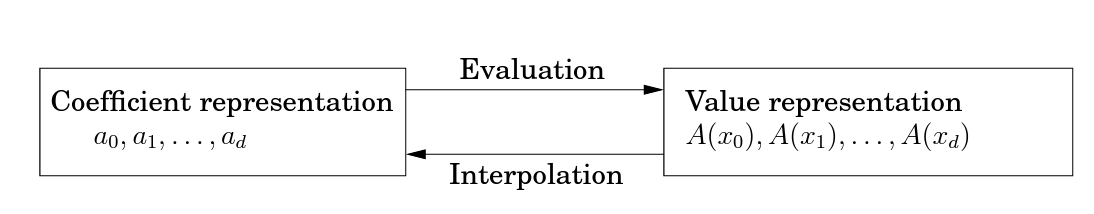
\includegraphics[scale=0.7]{images/poly-mult-algo.png}
    \caption{The resulting algorithm}
\end{figure}

How efficient is this? We'll the $d + 1$ selection of evaulation points and multiplication is just linear time. But how about when we evaluate the polynomials at the $d + 1$ points? Evaluating a polynomial of degree $d \le n$ at a single point is $\O(n)$ steps. Therefore the baseline for n points is $\Theta(n^2)$.

\begin{lemma}[Runtime of Evaluating a Polynomial at a Single Point]
    Suppose we are given a polynomial of degree $n - 1$: $p(x) = p_o + p_1 x + \dots + p_{n - 1} x^{n - 1}$

    \begin{align*}
        p(\alpha) & = p_0                                        &  & \text{0 mults}       \\
                  & + p_1 \alpha                                 &  & \text{1 mults}       \\
                  & + p_2 \alpha \cdot \alpha                    &  & \text{2 mults}       \\
                  & + p_3 \alpha \cdot \alpha \cdot \alpha       &  & \text{3 mults}       \\
                  & \dots                                                                  \\
                  & + p_{n - 1} \alpha \cdot \alpha \dots \alpha &  & \text{n - 1 mults}   \\
        \hline                                                                             \\
                  & p(a)                                         &  & \O(n^2) \text{mults}
    \end{align*}
    However notice that we are doing redundant work in each step. We already compute $\alpha^2$ in the second step, so we don't need to compute it again in the next step.

    With this, we can instead do each step in 1 multiplication by initializing an array where $A[i] = \alpha \cdot A[i - 1]$. So evaluating a polynomial takes $\O(n)$

\end{lemma}

\textbf{Fast Fourier Transform} is able to do the evaluation step in just $\O(n \log n)$, for a particular clever choice of $x_0, \dots , x_{n - 1}$, using \textbf{complex numbers.}

\subsubsection{Complex Numbers}
\begin{definition}[complex number]
    a number that's in the form:
    $$
        a + b \cdot i
    $$
    Where $a$ is called the real part, and $b$ is called the imaginary part and $i = \sqrt{-1}$
\end{definition}

\begin{figure}[H]
    \centering
    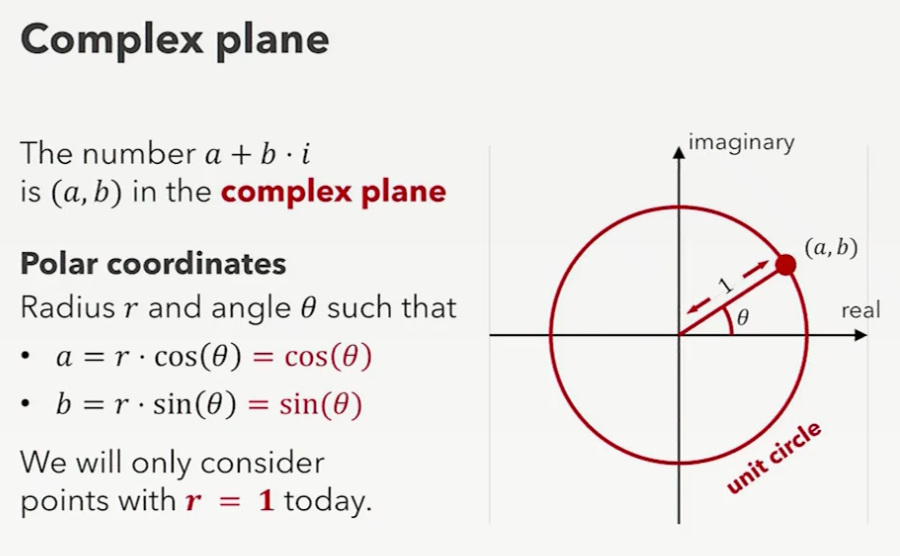
\includegraphics[scale=0.3]{images/complex-plane.png}
    \caption{Complex Plane}
\end{figure}

\subsubsection*{Roots of Unity}
\begin{itemize}
    \item \textbf{Unity} is just a fancy word for the number 1
    \item $n^{th}$  roots of unity = \{solutions to $x^n = 1$\}
    \item it's a point x where you raise it to the nth power and you get 1.
\end{itemize}

\begin{example}[Roots of Unity]
    \begin{itemize}
        \item $2^{nd}$ roots of unity = $\sqrt{1} = \{\pm 1\}$
        \item $4^{th}$ roots of unity = $\sqrt[4]{1} = \{\pm 1, \pm i\}$
        \item $8^{th}$ roots of unity =$\sqrt[8]{1} = \{\pm 1, \pm i, \pm \left(\dfrac{1 + i}{\sqrt{2}}\right), \pm \left(\dfrac{1 - i}{\sqrt{2}}\right)\}$
    \end{itemize}

    In general, the nth root of unity is n distinct numbers.
\end{example}
Visually, the {\color{red} nth} roots of unity is the {\color{red} n} \emph{equally} spaced points on the unit circle


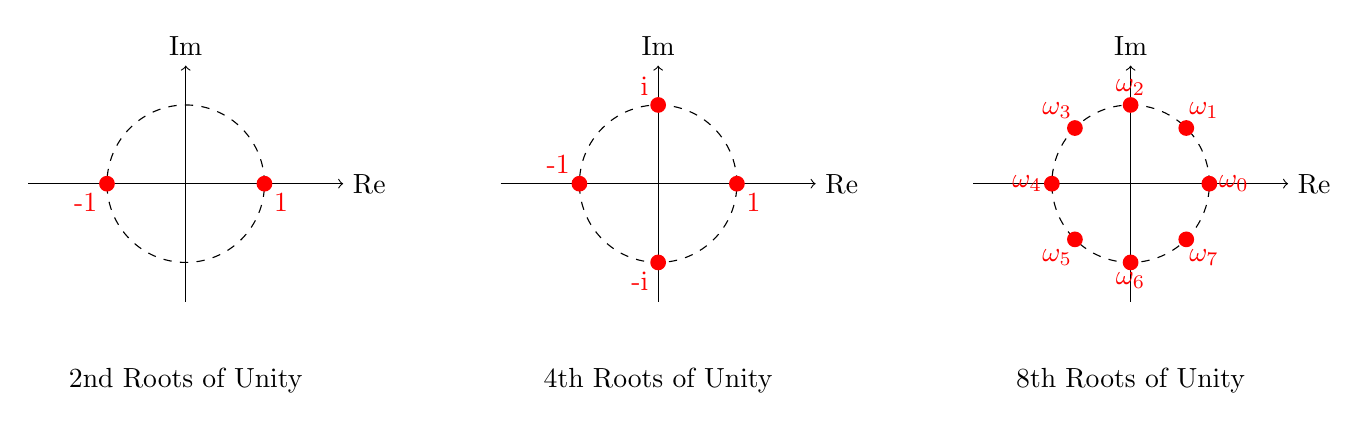
\begin{tikzpicture}
    % 2nd roots of unity
    \draw[->] (-2,0) -- (2,0) node[right] {Re};
    \draw[->] (0,-1.5) -- (0,1.5) node[above] {Im};
    \draw[dashed] (0,0) circle (1);
    \fill[red] (1,0) circle (0.1) node[below right] {1};
    \fill[red] (-1,0) circle (0.1) node[below left] {-1};
    \node at (0,-2.5) {2nd Roots of Unity};

    % 4th roots of unity
    \begin{scope}[xshift=6cm]
        \draw[->] (-2,0) -- (2,0) node[right] {Re};
        \draw[->] (0,-1.5) -- (0,1.5) node[above] {Im};
        \draw[dashed] (0,0) circle (1);
        \foreach \angle/\label/\position in {0/1/below right, 90/i/above left, 180/-1/above left, 270/-i/below left} {
                \fill[red] (\angle:1) circle (0.1) node[\position] {\label};
            }
        \node at (0,-2.5) {4th Roots of Unity};
    \end{scope}

    % 8th roots of unity
    \begin{scope}[xshift=12cm]
        \draw[->] (-2,0) -- (2,0) node[right] {Re};
        \draw[->] (0,-1.5) -- (0,1.5) node[above] {Im};
        \draw[dashed] (0,0) circle (1);
        \foreach \angle/\idx [count=\i from 0] in {0/0, 45/1, 90/2, 135/3, 180/4, 225/5, 270/6, 315/7} {
                \fill[red] (\angle:1) circle (0.1) node[anchor=\angle+180] {\(\omega_{\idx}\)};
            }
        \node at (0,-2.5) {8th Roots of Unity};
    \end{scope}
\end{tikzpicture}

Recall that when we multiply two complex numbers, we just add their angles, so we can come up with this formula.\\

\begin{lemma}[Formula for nth roots of unity]
    Formula: {\color{red} $n^{th}$} roots of unity
    \begin{align*}
        = \text{angle } 0 \cdot \theta, 1 \cdot \theta, 2 \cdot \theta, \dots &  & \text{where } \theta = \frac{2\pi}{n}
    \end{align*}

\end{lemma}


\begin{figure}[H]
    \centering
    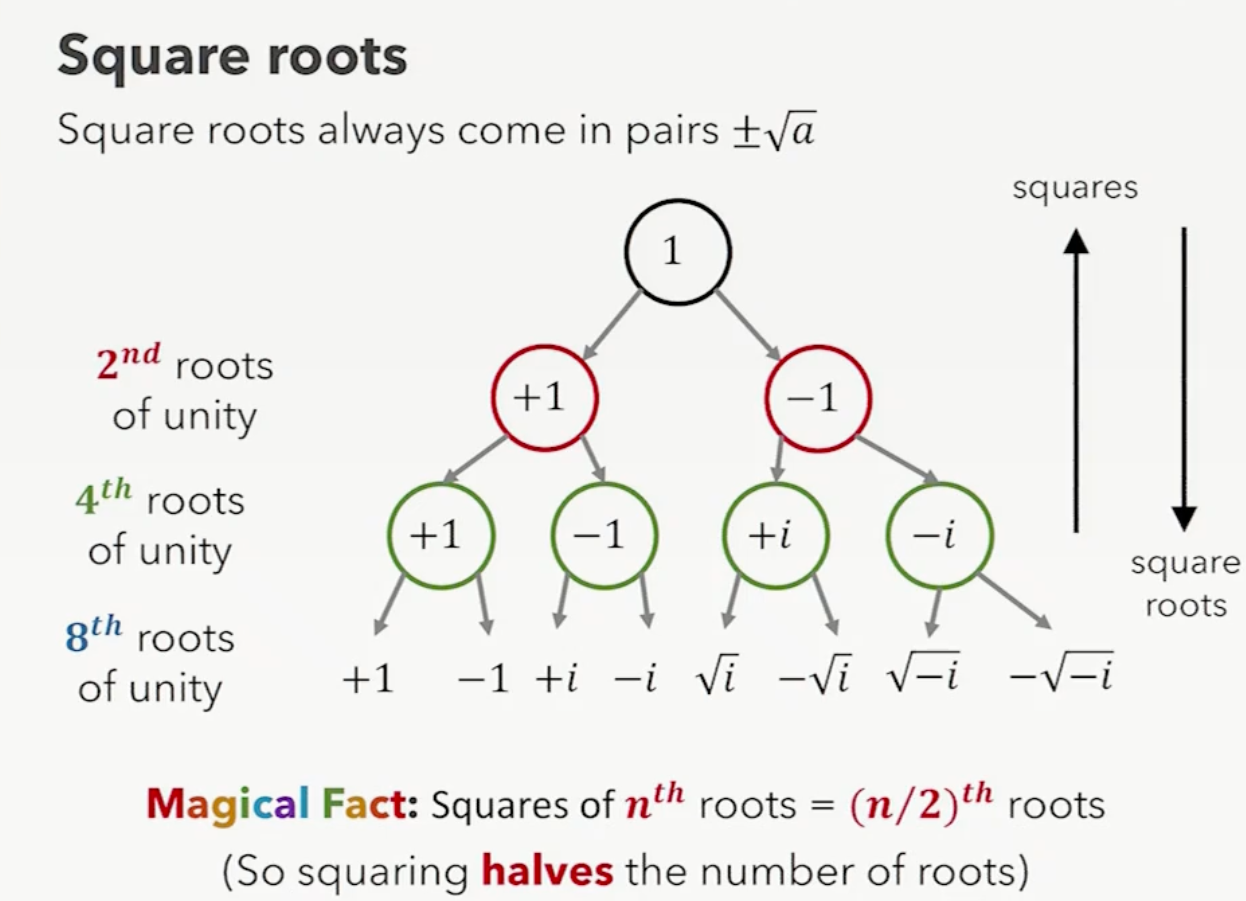
\includegraphics[scale=0.3]{images/unity.png}
    \caption{}
\end{figure}

\subsubsection*{Complex number Takeaways}
\begin{itemize}
    \item Generator fact: for all $0 \le i \le m - 1, \omega_i = \omega_1^i$
    \item The magical fact above
\end{itemize}



\lecture[09/10/23]{Polynomail Multiplication}
Recall that we are given two polynomials in their coefficient representation, and we want to compute their product. We saw last lecture that we can multiply two polynomials in their coefficient representation in $O(n^2)$

And also multiplying two polynomials in the value presentation takes $\O(n)$ time so it's optimal.


The bottle neck in the polynomial multiplication is the evaluation of the polynomials at $\O(n)$ points, which with the naive algorithm takes $\O(n^2)$ time. Can we possibly do this faster with a more clever choice of evaluation points? Yes

Lets design the algorithm:

Recall that if the degree of the polynomials we are multiply is of degree $n - 1$, then their product $C(x)$, has degree $2(n - 1) = 2n - 2$. Therefore in the value representation, $C(x)$ is defined by $2n - 1$ points. This means that we'll need to evaluate $p$ and $q$ on at least $2n - 1$ points, call it $m$, since we will be multiplying the values the polynomials to get $C(x)$


Let $m$ be the first power of 2 such that $m \ge 2n - 1$. We will evaluate p and q on {\color{red} $m^{th}$} roots of unit
$$
    {\omega_0, \omega_1, \dots, \omega_{m - 1}}
$$
in time $\O(m \log(m)) = \O(nlog(n))$. This is the \textbf{Fast Fourier Transform.}

\subsection*{Fast Fourier Transform}
The fast fourier transform is an algorithm for evaluating a polynomial of degree $n - 1$ on $m$ points in $\O(n\log n)$
\textbf{inputs:}
\begin{enumerate}
    \item $m$, a power of two
    \item a polynomial: $p(x) = p_0 + p_1 x + p_2 x^2 + \dots + p_{m-1}x^{m - 1}$
\end{enumerate}
\textbf{output }: $[p(\omega_0), p(\omega_1), \dots, p(\omega_{m - 1})]$


\subsubsection*{Divide an Conquer}
Let's write out $p(x)$ and split it into two parts, the evan part and odd part.
$$
    p(x) = p_0 + p_1 x + p_2 x^2 + \dots + p_{m-1}x^{m - 1}
$$

\begin{align*}
    \text{\textbf{even part: }}   & p_0 + p_2x^2 + p_4x^4 + \dots + p_{m - 2}x^{m - 2}                \\
                                  & p_0 + p_2x^2 + p_4(x^2)^2 + p_6(x^2)^3 + \dots                    \\
                                  & \text{\textbf{Even}}(x^2)                                         \\
    \text{where \textbf{Even}}(z) & = p_0 + p_2z + p_4z^2 + p_6z^3 + \dots                            \\
    .                                                                                                 \\
    \text{\textbf{odd part: }}    & p_1x + p_3x^3 + p_5x^5 + p_7x^7 + \dots + p_{m - 1}x^{m - 1}      \\
                                  & =x\cdot(p_1 + p_3x^2 + p_5x^4 + x^6 + \dots + p_{m - 1}x^{m - 1}) \\
                                  & =x \cdot \text{\textbf{Odd}}(x^2)                                 \\
    \text{ where \textbf{Odd}}(z) & = p_1 + p_3z + p_5 z^2 + \dots                                    \\
    .                                                                                                 \\
    \therefore p(x) = \text{Even}(x^2) + x \cdot \text{Odd}(x^2)                                      \\
    \text{where deg(\textbf{Even})} = \frac{m - 2}{2} = \frac{m}{2} - 1 \text{, same for deg(\textbf{Odd})}
\end{align*}

Recall what the goal is: we need to to evaluate the polynomial at $m$ points, which will be the $m^{th}$ roots of unity. We choose the $m^{th}$ roots of unity because it has $m$ solutions, $\omega_0, \dots \omega_{m - 1}$
$$
    [p(\omega_0), p(\omega_1), \dots, p(\omega_{m - 1})]
$$

$$
    p(\omega_i) = p_e(\omega_i^2) + \omega_i p_o(\omega_i^2)
$$
The recurrence relation we therefore get is as follows:
$$
    T(m) = 2T(m / 2) + \O(m)
$$

Which is $\O(n\log n )$ by the masters theorem. Next up is interpolation. How can we do it in $\O(n\log n)$?
\subsection*{Faster Interpolation}
The algorithm input is a polynomial at $m$ values, and output the coefficient of that polynomials.

\subsection*{Interpolation (Inverse FFT)}
Here is an idea for how to pick the $m$ points at which to evaluate a polynomial $A(x)$ of degree $\le n - 1$. If we choose them to be positive-negative pairs, that is:

\textbf{FT formula:}
$$
    p(\omega_l) = \sum_{j = 0}^{m - 1} p_j \cdot (\omega_l)^j
$$

\textbf{Inverse FT Formula:}
\begin{align*}
    p_l & = \frac{1}{m} \cdot \sum_{j = 0}^{m - 1} p(\omega_j) \cdot (\omega_{m - l})^j \\
        & = \frac{1}{m} \cdot q(\omega_{m - l})
\end{align*}



\subsubsection*{The matrix viewpoint}
Recall we have a polynomial and we compute it's values at m points, which are the roots of unity.
$$
    p(x) = p_0 + p_1 x + p_2 x^2 + \dots + p_{m-1}x^{m - 1}
$$



$$
    \pm x_0, \pm x_1, \dots , \pm x_{n/2 - 1}
$$

\begin{align*}
    \begin{bmatrix}
        p(\omega_0) \\
        p(\omega_1) \\
        p(\omega_2) \\
        \vdots      \\
        p(\omega_{m - 1})
    \end{bmatrix}
     & =
    \begin{bmatrix}
        \begin{array}{cccc}
            p_0 & + p_1 \omega_0     & + p_2 \omega_0^2     & + \dots + p_{m-1}\omega_0^{m - 1}     \\
            p_0 & + p_1 \omega_1     & + p_2 \omega_1^2     & + \dots + p_{m-1}\omega_1^{m - 1}     \\
            p_0 & + p_1 \omega_2     & + p_2 \omega_2^2     & + \dots + p_{m-1}\omega_2^{m - 1}     \\
                & \vdots             &                      &                                       \\
            p_0 & + p_1 \omega_{m-1} & + p_2 \omega_{m-1}^2 & + \dots + p_{m-1}\omega_{m-1}^{m - 1}
        \end{array}
    \end{bmatrix}
    \\
     & =
    \underbrace{\begin{bmatrix}
                        1      & \omega_0     & \omega_0^2     & \dots  & \omega_0^{m - 1}     \\
                        1      & \omega_1     & \omega_1^2     & \dots  & \omega_1^{m - 1}     \\
                        1      & \omega_2     & \omega_2^2     & \dots  & \omega_2^{m - 1}     \\
                        \vdots & \vdots       & \vdots         & \ddots & \vdots               \\
                        1      & \omega_{m-1} & \omega_{m-1}^2 & \dots  & \omega_{m-1}^{m - 1}
                    \end{bmatrix}}_{M}
    \underbrace{\begin{bmatrix}
                        p_0    \\
                        p_1    \\
                        p_2    \\
                        \vdots \\
                        p_{m - 1}
                    \end{bmatrix}}_{[p]}
\end{align*}
This is called a \textbf{Fourier Transform Matrix}. Naively, this matrix vector product computes in $O(m^2)$, but FFT solves this problem in $\O(m\log m)$ time.

\textbf{Note:} it solves this \textbf{without ever writing down $M$}


\textbf{Inverse Fourier Transform:}
We start off with the values of a polynomial at m points and want the coefficients of a polynomial.

\begin{align*}
    M^{-1} \cdot \begin{bmatrix}
                     p(\omega_0) \\
                     p(\omega_1) \\
                     p(\omega_2) \\
                     \vdots      \\
                     p(\omega_{m - 1})
                 \end{bmatrix}
    = \begin{bmatrix}
          p_0    \\
          p_1    \\
          p_2    \\
          \vdots \\
          p_{m - 1}
      \end{bmatrix}
\end{align*}

Then the computations required for each $A(x_i)$ and $A(-x_i)$ overlap a lot, because the even powers of $x_i$ coincide with those of $-x_i$.

\lecture[]{}
\lecture[]{}
\lecture[]{}
\lecture[]{}
\lecture[09/12/23]{Paths in Graphs}
\lecture[]{}
\lecture[10/5/23]{Dynamic Programming Pt 1}
\subsection{Elements of Dynamic Programming}
Dynamic programming is a powerful algorithmic paradigm in which a problem is solved by identifying a collection of subproblems and tackling them on by one, smallest first, using the answers to small subproblems to help figure out larger one, until the whole lot of them is solved.

Large problems break up into smaller sub problems, i.e., the solution of some big problem can be expressed in terms of the solutions to the smaller sub-problems.
\begin{quotation}
    eg. fib(n) = fib(n - 1) + fib(n - 2)
\end{quotation}
But what's different about dynamic programming from divide and conquer? After all in divide and conquer we also solved smaller subproblems. The problems that are solved with dynamic programming have a lot of overlapping subproblems. This means that we can save resources by solving a subproblem once and storing its value, and then use that subproblem many times over.

\begin{quotation}
    eg. fib(i + 1), fib(i + 2), ... All use fib(i) indirectly, so we can store the value of fib(i) instead of having to repeatedly compute it.
\end{quotation}

\subsubsection{Here is a general template to solve DP problems}
\begin{itemize}
    \item \textbf{step 1:} Identify subproblems. What makes a good subproblem?
          \begin{itemize}
              \item Not too many of them (the more subproblems the slower the DP algorithm is).
              \item Must have enough information in it to compute subproblems recursively. (needed for step 2.)
          \end{itemize}
    \item \textbf{step 2:} Find a recursive formulation for the subproblems
    \item \textbf{step 3:} Design the dynamic programming algorithm and memoize computation starting from the smallest subproblems and build up
\end{itemize}

\subsection{Two ways to do DP}
\begin{itemize}
    \item \textbf{Top Down}: start from the biggest problem and recurse to smaller problems. Looks just like recursion, with one exception: \textbf{memoization}; keeping track of what smaller problems we have solved already.
    \item \textbf{Bottom up:} start from the smallest problems first and then bigger problems. Still memo-ize, but usually doesn't have a recursive call.
\end{itemize}

\subsubsection{Fibonacci Numbers}
Recall the naive recursive way to compute fibonacci:
\begin{lstlisting}
    def fib(n):
        if n <= 1:
            return n
        else:
            return fib(n - 1) + fib(n - 2)
\end{lstlisting}
The runtime of this algorithm is exponential, extremely slow. The first observation we can make about why this algorithm is so slow is that the recursion tree repeats a lot of sub-problems. For every node, in the recursive tree, it recomputes the problem from scratch.

\begin{figure}[H]
    \centering
    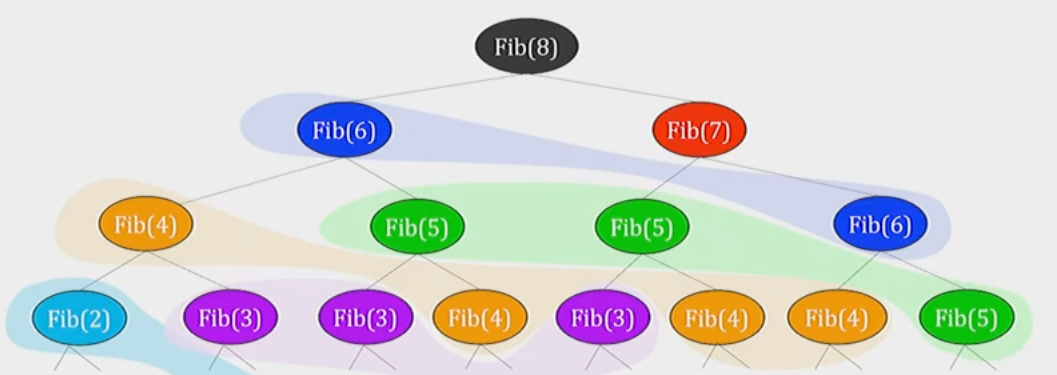
\includegraphics[scale=0.4]{images/fib-recursive-tree.png}
    \caption{Repetition in fib recursion tree}
\end{figure}

So how can we fix this? We can keep an array and remember the computation we did so that we don't have to recompute this in another subproblem (\textbf{memo-ization}).

\begin{lstlisting}
    memo = [0, 1, None, None, ..., None] # Global array

    def fastFibTopDown(n):
        if memo[n] != None:
            return memo[n]
        else:
            mem[n] = fastFibTopDown(n - 1) + fastFibTopDown(n - 2)
            return mem[n]
\end{lstlisting}

We can also do a bottom up.

\begin{lstlisting}
        def fastFibBottomUp(n):
            mem = [None] * (n + 1)
            mem[0] = 0
            mem[1] = 1
            for i in range(2, n + 1):
                mem[i] = mem[i - 1] + mem[i - 2]
            return mem[n]
\end{lstlisting}

An additional optimization we can make with this approach to the space complexity. Notice that in fib, we only need to keep track of the two previous elements (f(n - 1), f(n - 2)), so we instead of keeping track of all fib values from 0...n, lets only keep track of the two previous values so that we can compute the next value.
\begin{figure}[H]
    \begin{lstlisting}
            def fibBottomUpSpaceSaving(n):
                mem = [0, 1]
                for i in range(2, n + 1):
                    x = mem[0] + mem[1]
                    mem[0] = mem[1]
                    mem[1] = x
                return mem[1]
        \end{lstlisting}

\end{figure}

\subsection{DP order of Computation and Dags}
There is an implicit DAG in dynamic programming problems! The nodes are the subproblems we define, and its edges are the dependencies between the subproblems: if to solve subproblem $B$, we need the answer to subproblem $A$, then there is a conceptual edge from $A$ to $B$.

To see this for fib, lets draw a directed edge (i, j) if the computation of i directly depends on/uses the solution to subproblem j.

BottomUp solves problems in the order (or reverse order, depending on how you drew edges, in this draw it's reverse order) of this topological sort.

In Top Down: we starting recursing at the top, but but the memo the memo-ization table starts to get filled according to the reverse topological sort graph.

\begin{figure}[H]
    \begin{center}
        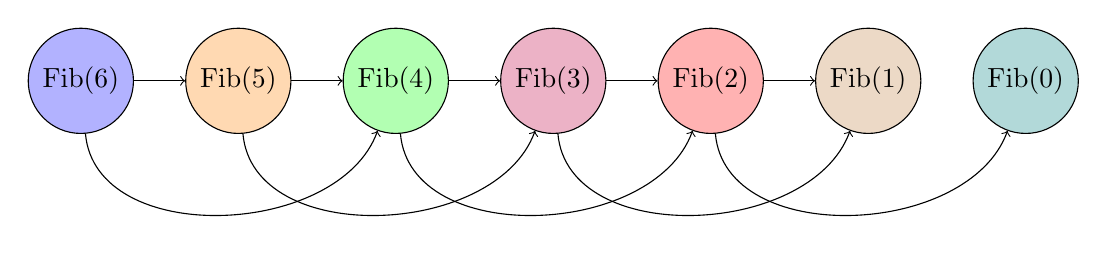
\begin{tikzpicture}
            % Nodes
            \node[draw, circle, fill=blue!30] (fib6) at (0,0) {Fib(6)};
            \node[draw, circle, fill=orange!30] (fib5) at (2,0) {Fib(5)};
            \node[draw, circle, fill=green!30] (fib4) at (4,0) {Fib(4)};
            \node[draw, circle, fill=purple!30] (fib3) at (6,0) {Fib(3)};
            \node[draw, circle, fill=red!30] (fib2) at (8,0) {Fib(2)};
            \node[draw, circle, fill=brown!30] (fib1) at (10,0) {Fib(1)};
            \node[draw, circle, fill=teal!30] (fib0) at (12,0) {Fib(0)};

            % Connections
            \draw[->] (fib6) -- (fib5);
            \draw[->] (fib6) to[out=275,in=250] (fib4);
            \draw[->] (fib5) -- (fib4);
            \draw[->] (fib5) to[out=275,in=250] (fib3);
            \draw[->] (fib4) -- (fib3);
            \draw[->] (fib4) to[out=275,in=250] (fib2);
            \draw[->] (fib3) -- (fib2);
            \draw[->] (fib3) to[out=275,in=250] (fib1);
            \draw[->] (fib2) -- (fib1);
            \draw[->] (fib2) to[out=275,in=250] (fib0);
        \end{tikzpicture}
        \caption{Fib(6) drawn as a DAG}
    \end{center}
\end{figure}


\subsection{SSSP on DAG's}
Recall the shortest paths problem on dags. We're given a weighted graph $G$ (positive or negative weight)  and a starting vertex $s$, and want to compute the shortest path to every vertex $u$ from $s$. How do we do that?

\begin{align*}
    f(u) = \text{length of shortest path from s to u} \\
    f(u) = \begin{cases}
               0,                                          & \text{if } u = s         \\
               \infty,                                     & \text{elif indeg}(u) = 0 \\
               \min\limits_{(v, u) \in E}{f(v) + w(v, u)}, & \text{otherwise}
           \end{cases}
\end{align*}

The recursive case takes the minimum path from every edge coming to u + the weight of the edge. But how do we code this?

In code we are given an adjacency list, a list where the linked list contains all the outgoing edges of the current vertex, we want all the incoming edges though, so we reverse the graph.

\subsection{Bellman Ford}
\begin{lstlisting}
    def Bellman(G, s):
        T[1...n] = all infinity
        T[s] = 0
        for k = 1 to |V| - 1:
            for e = (u, v) in E:
            $\frac{1}{2}$
                T[v] = min{T[v], T[u] + w(u, n)}
        return T;
\end{lstlisting}

The first step in figuring out the solution to a DP problem is to find a function that has a nice recurrence relation that we can then memoize. So what is the function that we are gonna use that will eventually lead us to solve bellman ford?

\begin{itemize}
    \item $f(b,k) =$ length of shortest path from $s \rightarrow b$ using $\le$ edges
    \item since we can assume that the shortest path without a negative cycle connecting that shortest path cannot use more than n - 1 edges, otherwise if it did then it would not be a tree, i.e., there is a cycle. So we want $f(t, n - 1)$
    \item $$f(b, k) = \begin{cases}
                  0,                                                                    & b = s, k = 0     \\
                  \infty,                                                               & b \neq s, k = 0  \\
                  \min(f(b, k - 1), \min\limits_{(v, b) \in E}(f(v, k - 1) + w(v, b))), & \text{otherwise}
              \end{cases}
          $$
\end{itemize}
To understand this recurrence relation, lets explain the three cases.
\begin{itemize}
    \item The first case is when $b = s$ and we use no edges, therefore we've already reached b.
    \item The second case is when $b \ne s$ and we use no edges, therefore it's impossible to get to b since we cannot use any more edges.
    \item The third case is best explained by picture. The first term in the argument of min is $f(b, k - 1)$ since certainly if we are allowed to use at most $k$ edges, then are allowed to try and get to $b$ with $k - 1$ edges. The second term is another min: $\min\limits_{(v, b) \in E}(f(v, k - 1) + w(v, b))$ which is best explained by the picture below:
\end{itemize}
\begin{center}
    \begin{tikzpicture}
        \draw[->] (0,0) node[left] {$s$} -- (1,1);
        \draw[->] (1,1) -- (2,0);
        \draw[->] (2,0) -- (3,1) node[above] {$v$};
        \draw[->] (3,1) -- (4,0) node[right] {$b$};
    \end{tikzpicture}
\end{center}

Take the previous edge of to $b$ with the minimum shortest distance + the weight of that edge.

\subsection{All Pair Shortest Paths Algorithm}
This algorithm output should be a 2d-array ($n \times n$) $T[1\dots n][1 \dots n]$, s.t. $T[i][j] = $ length of shortest path from node $i$ to node $j$.

The naive solution would be to run bellman ford from every vertex. What's the runtime? Each run of bellman ford takes $\O(nm)$, and you run it n times, so in total this algorithm has runtime: $\O(n^2m)$ which is potentially $\O(n^4)$ if the graph is dense.

We'll discuss a faster algorithm (\emph{Floyd Warshall}) that has runtime $\O(n^3)$

\begin{lstlisting}
    def FloydWarshall(G):
        init $T[1 \dots n][1 \dots n] = $ all $\infty$
        for each vertex i to n:
            T[i][i] = 0

        for each edge (u, v) $\in E$:
            T[u][v] = w(u, v)

        for k = 1 to n:
            for i = 1 to n:
                for j = 1 to n:
                    a = T[i][j]
                    b = T[i][k] + T[k][j]
                    T[i][j] = min(a, b)
        return T
\end{lstlisting}

let $f(i, j, k) = $ length of shortest path from i to j using intermediate vertices that must be in the set $\lbrace1, ..., k \rbrace$

$$f(i, j, k) =
    \begin{cases}
        0,       & \text{if } i = j, k = 0    \\
        w(i, j), & \text{if } i \neq j, k = 0 \\
        \min \left\{
        \begin{array}{c}
            f(i,j,k-1),             \\
            f(i,k,k-1) + f(k,j,i-1) \\
        \end{array}
        \right\} & \text{otherwise }
    \end{cases}$$

The recurrence relation is best explained by the picture in DPV. There are two cases, the shortest path from i to j is better than the shortest path i to k + 1 and the k + 1 to j.


\lecture[10/10/23]{Dynamic Programming Pt 2}
Agenda for this lecture:
\begin{itemize}
    \item Longest Increasing Subsequence
    \item Edit Distance
    \item Knapsack
\end{itemize}

\subsection{Longest Increasing Subsequences}
\begin{itemize}
    \item \textbf{input}: an array of $n$ integers $a = [a_1, \dots, a_n]$
    \item \textbf{output}: The length of the longest increasing subsequence, not necessarily contiguous, of the input.
\end{itemize}
Subproblem: let $L[j] =$ length of LIS in the array $[a_1, \dots, a_j]$ that \textbf{ends in $a_j$} for $j = 1, ..., n$.

Why must it end in $a_j$? Because how else would we know that we can add a new element to the subsequence? The next element must be greater than $a_j$, the largest element so far in the current subsequence.

This gives us a recursive formula:

$$
    L[j] = 1 + \max\limits_{i < j}(L[i]  \mid a_i < a_j)
$$

The pseudo code will be as follows:
\begin{lstlisting}
    def LIS(a):
        L[1...n] = all 0
        for j = 1 to n:
            best = 0
            for i = 1 to j:
                if $a_i < a_j$:
                    best = max(best, $L[i]$)
            L[j] = 1 + best
    return max(L)
\end{lstlisting}
It's easy to see that the runtime of this is $\O(n^2)$.

\subsection{Edit Distance}
\begin{itemize}
    \item \textbf{input}: two strings $S[1\dots m]$ and $T[1\dots n]$
    \item \textbf{output}: compute the smallest number of edits to turn S into T.
\end{itemize}
The edits that are allows are:
\begin{enumerate}
    \item insert a character into S
    \item delete a character from S
    \item change on character to another character
\end{enumerate}
Applications of edit distance:
\begin{itemize}
    \item auto correct
    \item word suggestions in search engines
    \item dna analysis of similarities
\end{itemize}
\subsubsection*{Defining the subproblem}
For all $0 \le i \le m$ and $0 \le j \le n$, let:

$$
    E(i, j) = \text{EditDist}(S[1\dots i], T[1\dots j])
$$
Be the cost of optimal alignment between $S[1\dots i], T[1\dots j]$. How many subproblems do we have? We have a subproblem for every $i, j$ pairs, each having $m + 1$ and $n + 1$ different possible numbers respectively, therefore we have $\O(m\cdot n)$ subproblems.

\subsubsection{Finding the Recurrence relations}.
What are the three ways of aligning $S[1\dots i]$ and $T[1 ... j]$ using the smaller subproblems. There are three ways to do this.
\begin{enumerate}
    \item Case 1: $S[i]$ is deleted, (aligned with an empty space in T)
    \item Case 2: $T[j]$ is added.
    \item Case 3: Change $S[i]$ to $T[j]$
\end{enumerate}
\begin{align*}
    E(i, j) =
    \min \left\{
    \begin{array}{c}
        1 + E(i - 1, j),    \\
        1 + E(i, j - 1),    \\
        1 + E(i - 1, j - 1) \\
    \end{array}
    \right\}
\end{align*}
The bases cases are when we align the a string with an empty string, which has an alignment cost of the non empty string since we'd have to delete that many characters to align them. Therefore: $E(0, j) = j$ and $E(i, 0) = i$.

\textbf{What's the runtime?} Each subproblem relies on only 3 smaller subproblems, which could be computed first to and memoized. There are $\O(mn)$ subproblems, and each does an $\O(1)$ operation, therefore the runtime is $\O(mn)$

\subsection{Knapsack With Repetition}
\textbf{input}: a weight capacity $W$, and $n$ items with (weights, values): $(w_1, v_1), \dots , (w_n, v_n)$.

\textbf{output:} Most valuable combination of items, whose total weight is at most $W$.

\textbf{Two Variants: }
\begin{enumerate}
    \item With repetition (aka unbounded supply, aka with replacement), i.e., for each item $i$, we can take as many copies of it as we want.
    \item Without repetition (0-1 knapsack, aka without replacement), i.e., for each item $i$, we either take 1 copy or 0 copy of it.
\end{enumerate}

\subsection{With Repetition}
\textbf{Defining a subproblem:} for all $c \le W, \text{ let } K(c) = $ best value achievable for knapsack of capacity $c$.

\textbf{Recurrence relation: } How can we write $K(c)$ interms of smaller subproblems? Well if $K(c)$ includes item $i$, then removing it would give us an optimal solution to $K(c - w_i)$. Therefore $K(c) = K(c - w_i) + v_i$ for some item $i$. We don't know which item so we need to try all possibilities:

$$
    K(c) = \max \limits_{i : w_i \le c}(v_i + K(c - w_i))
$$

\begin{lstlisting}
    def KnapSackWRepetition(W, $(w_1, v_1), \dots , (w_n, v_n)$)
        init K to array of size W + 1
        K(0) = 0 # bag with zero capacity has no value.
        for $c$ = 1 to W:
            K($c$) = $\max \limits_{i : w_i \le c}(v_i + K(c - w_i))$
        return K(W)
\end{lstlisting}

\subsubsection{Analying Runtime:}
How many subproblems do we have? $O(W)$, we start from 0 and go all the way to $W$

How much work do we do per subproblem? We take a max of at most $n$ items, therefore $\O(n)$ time per subproblem.

Total runtime = $\O(Wn)$

\subsection{Knapsack Without Repetition}
\textbf{input: } same input as above

\textbf{output: } most valuable \underline{subet of items}, whose total weight is $\le W$.


Without repetition, our previous subproblem now becomes completely useless. Knowing the value of $K(c - w_i)$ is the maximum value doesn't help us, since we don't know whether or not item $n$ already got used up in this partial solution. We must refine our subproblem to carry additional information about the items being used.

\subsubsection{Finding a subproblem}
\textbf{Idea:} Solve knapsack for smaller capacities and \textbf{also} smaller set of items.
We add a second parameter $0 \le j \le n$.
$$
    K(c, j) = \text{max value achievable using a knapsack of capacity w and items } 1, \dots, j.
$$
The answer we seek is $K(W, n)$.
\subsubsection{Find Recurrence Relation}
How can we write $K(c, j)$ in terms of smaller subproblems? There are two cases.
\begin{itemize}
    \item Case 1: Opt sln using items $1, ..., j$ doesn't actually use item $j$.
    \item Case 2: Opt sln using items $1, \dots, j$ uses item $j$.
\end{itemize}
Therefore we take the best (max) of these two cases
\begin{align*}
    K(c, j) = \max \left\{
    \begin{array}{c}
        K(c, j - 1), \\
        K(c - w_j, j - 1) + v_j.
    \end{array}
    \right\}
\end{align*}

\subsubsection{Designing the Algorithm}
How do we memo-ize the subproblems in this recurrence relation?

The bases cases are as follows:
\begin{itemize}
    \item $K(c, 0) = 0$, since we aren't allowed to use any items.
    \item $K(0, j) = 0$, since we no don't have capacity for more items.
\end{itemize}
What's the memoization order? We should be thinking about the subproblems as a 2d array. If the columns of this table is the weights, and the rows is the items, each subproblem relies on the previous row, $K(c, j - 1)$, which is directly above it, and $K(c - w_j, j - 1)$, which is also above it, but somewhere to the left.
\begin{figure}[H]
    \centering
    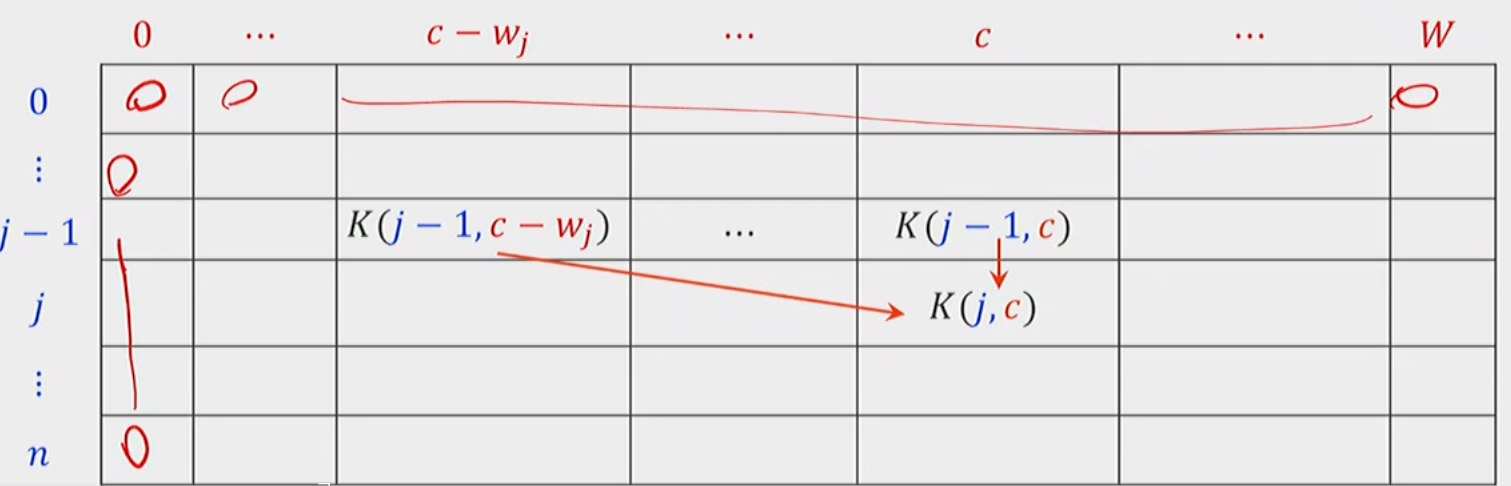
\includegraphics[scale=0.3]{images/knapsack-without-repetition-memoization.png}
    \caption{Memoization order}
\end{figure}
\subsubsection{Runtime of this algorithm}
There is $\O(W\cdot n)$ subproblems. Each subproblem consists of taking a max over 2 values, therefore $\O(1)$ time per subproblem.

Therefore, the total runtime is: $\O(W\cdot n)$ runtime. (.\emph{pseudo polynomial time alg})

\textbf{Space complexity}: we can naively store a 2d array, but notice we only need the previous row to compute the current subproblem. Therefore we only need to store $\O(W)$ amount of space; the current row, and the previous row.

\lecture[10/12/23]{Dynamic Programming Pt.3}
\subsection{Traveling Salesman Problem}
\textbf{Input: } cities $1\dots n$ and pairwise distances $d_{ij}$ between cities $i$ and $j$. (a fully connected graph)

\textbf{Output: } Find a "tour" of minimum total distance.

\begin{definition}[Tour]
    A tour is a path through the cities, that
    \begin{enumerate}
        \item starts from city 1
        \item visits every city, exactly once
        \item returns to city 1.
    \end{enumerate}
\end{definition}

\subsubsection{Finding a Subproblem}
Suppose we started at city 1 as required, have visited a few cities, and now in city $j$. What information do we need in order to extend this partial tour? We certainly need to know $j$, since this will determine which cities are most convenient to visit next. And we also need to know all the cities visited so far, so that we don't repeat any of them.

Subproblems refer to partial solutions, and in this case, the most obvious partial solution is the initial portion of a tour. It starts from city 1, ends in city $j$, passing through all cities in a set $S$ (which includes 1 and $j$)

\textbf{Subproblems: } for all $j \le n$ and $S \subseteq \{1, \dots, n\}$, s.t.  $S$ includes $1$ and $j$, let
$$
    T(S, j) = \text{length of the shortest path visiting all cities in } S \text {exactly onces starting from 1 and ending at }j.
$$

\subsubsection{Finding the Recurrence Relation}
How can we compute $T(S, j)$ using smaller subproblems? What should we pick as the second-to-last city before visiting $j$. It has to be some city in $S$, since we must pass it before visiting $j$. Let that city be $i$.

Therefore the overall length from $1$ to $j$ is $T(S - {j}, i) + d_{ij}$, we must pick the best such $i$:

\begin{align*}
    T(S, j) = \min\{T[S - \{j\}, i] + d_{ij} &  & \mid i \in S \land i \neq j\}
\end{align*}

What about the bases cases?
\begin{itemize}
    \item $T(\{1\}, 1) = 0$, since the distance starting at 1, and ending at 1, using only city 1, is 0, you don't move.
    \item For all other $|S| \ge 2$, $T(S, 1) = \infty$ since we don't wait a partial tour to start and end at the same city, our final solution will.
\end{itemize}

\textbf{Final solution: } Recall that we want to start and end at city $i$, therefore we want to find the best $j$, (the best city to end in) such that the cost is minimized, i.e.,
$$
    \min\limits_{j \neq 1} T(\{1,\dots , n\}, j) + d_{j1}
$$

\subsubsection{Designing the Algorithm}
\begin{lstlisting}
    def TSP(D):
        init array T of size $2^n \times n$ # $2^n$ different possible subsets $S$
        T[{1}, 1] = 0
        for set size s = 2 to n:
            for sets $S$ of size s and containing $1$:
                T[S, 1] = $\infty$
                for all $j \in S \land j \neq 1$:
                    $ T[S, j] = \min\limits_{i \in S \land i \neq j}\{T[S - {j}, i] + d_{ij}\}$
        return $\min\limits_{j \neq 1} T[\{1,\dots , n\}, j] + d_{j1}$
\end{lstlisting}
\subsubsection{Runtime anaylsis}
There is $2^n \cdot n$ subproblems and each takes linear time to solve. Therefore the total runtime is $\O(2^n\cdot n^2)$

\subsection{Independent Sets in Trees}
We consider independent sets in trees and not general graphs because this problem can't be in done polynomial time.

\textbf{Input:} Undirected graph $G = (V, E)$, which is a tree.

\textbf{Output:} Largest "independent set" of $G$. An independent set of $G$, is $S \subseteq V$, if there are no edges between any $u, v \in S$


\subsubsection{Finding the Subproblem:}
We can start by rooting the tree at any node $r$, which gives us a natural ordering of children, and grand children, etc, of the rooted node. Now, each nodes defines a subtree--the one hanging from it.

This immeditely suggests subproblems:

$$
    I(u) = \text{size of largest independent set of subtree hanging from} u.
$$
Our goal is to find $I(r)$.
\subsubsection{Finding a Recurrence Relation:}
There are two cases:
\begin{itemize}
    \item case 1: The independent set includes $u$.
    \item case 2: The independent set doesn't includes $u$.
\end{itemize}
Therefore the recurrence relation is as follows:

\begin{align*}
    I(u) = \max\left(\begin{array}{c}
                         1 + \sum\limits_{\text{grandchildren w of u}} I(w), \\
                         \sum\limits_{\text{children w of u}} I(w)
                     \end{array}\right)
\end{align*}


\lecture[]{Linear Programming}
\begin{example}
    Imagine there is a factory that produces two items, \emph{foo} and \emph{bar} with some ingredients to make. Foo sells for $\$4 / \text{oz}$ and bar sells for $\$5 / \text{oz}$.
    \begin{itemize}
        \item foo takes 1 oz butter, 2  oz water, and 4 oz goo
        \item bar takes 6 oz butter, 3 oz goo
    \end{itemize}
    The factory has a limited number of ingredients:
    \begin{itemize}
        \item W = 10 oz of water
        \item B = 6 oz of butter
        \item G = 6 oz of goo
    \end{itemize}
    How many foos and bars should the factory make to maximize profit? This could be modeled as a linear program. Here are the equations:

    \begin{align}
        \max 4x + 5y   &  & \text{Object: profit}                                    \\
        1x + 6y \le 6  &  & \text{butter constraint}                                 \\
        2x + 0y \le 10 &  & \text{water constraint}                                  \\
        4x + 3y \le 6  &  & \text{goo constraint}                                    \\
        x, y \ge 0     &  & \text{non negative production of foo and bar constraint}
    \end{align}

    The plot with these equations is as follows.
    \begin{center}
        \begin{tikzpicture}
            \begin{axis}[
                    xmin=0, xmax=3,
                    ymin=0, ymax=3,
                    xlabel={$x$ (foo)},
                    ylabel={$y$ (bar)},
                    grid=major,
                ]


                % Fill feasible region
                \fill[fill=red!10] (axis cs:0,0) -- (axis cs:0,1) -- (axis cs:0.0,1) -- (axis cs:0.9,0.83) -- (axis cs:1,0.7) -- (axis cs:1,0) -- cycle;

                % Add constraints
                \addplot[name path=butter, domain=0:3] {1 - x/6} node[pos=0.5, sloped, above] {butter};
                \addplot[name path=water, domain=0:3] {10/2} node[pos=0.5, sloped, above] {water};
                \addplot[name path=goo, domain=0:3] {2 - 4*x/3} node[pos=0.5, sloped, above] {goo};

                % Optimal point
                \coordinate (opt) at (axis cs:0.85,0.85);
                \node[circle, fill=red, inner sep=1.5pt] at (opt) {};
                \node[above right, rotate=35] at (opt) {Optimal Point};

                % Add axes labels
                \addplot[mark=none, color=black] coordinates {(0, 0) (0, 3)} node[pos=1, left] {$y$};
                \addplot[mark=none, color=black] coordinates {(0, 0) (3, 0)} node[pos=1, below] {$x$};

            \end{axis}
        \end{tikzpicture}
    \end{center}
    If we rotate this plot where the object function points in the z axis, and have a marble roll down this hill, it will end up at the optimal point.
\end{example}
\subsection{Simplex Algorithm}
The simplex algorithm is an algorithm that solves linear programs. It's a greedy algorithm that starts at a vertex in the feasible region, and then moves to a better vertex solution, until it can't move anymore.

It's a greedy algorithm because it always moves to a better solution, and it's a local search algorithm because it only looks at the neighbors of the current solution.

\end{document}